\documentclass[runningheads]{llncs}

\usepackage[T1]{fontenc}
\usepackage{graphicx}
\usepackage{amsmath}
\usepackage{amssymb}
\usepackage{booktabs}
\usepackage{multirow}
\usepackage{array}
\usepackage{url}
\usepackage{hyperref}
\usepackage{placeins}
\usepackage{algorithm}
\usepackage{algpseudocode}
\usepackage{tikz}
\usetikzlibrary{positioning,arrows.meta,calc,fit,shapes.geometric,backgrounds}
\usepackage{pgfplots}
\pgfplotsset{compat=1.17}
\usepackage{xcolor}
\definecolor{MidnightBlue}{HTML}{2c3e50}
\definecolor{DarkOrange}{HTML}{e67e22}
\definecolor{DarkOrchid}{HTML}{8e44ad}

% Tight spacing for page budget
\linespread{0.90}
\setlength{\abovecaptionskip}{3pt}
\setlength{\belowcaptionskip}{1pt}
\setlength{\textfloatsep}{4pt plus 1pt}
\setlength{\floatsep}{4pt plus 1pt}
\setlength{\intextsep}{4pt plus 1pt}
\setlength{\abovedisplayskip}{3pt plus 1pt}
\setlength{\belowdisplayskip}{3pt plus 1pt}

% Springer eBook style for hyperref
\usepackage{color}
\renewcommand\UrlFont{\color{blue}\rmfamily}
\urlstyle{rm}

\begin{document}

\title{Marginal-Carbon-Aware Deferral of Deadline-Elastic Serverless
Workloads in the Cloud--Edge Continuum}

\titlerunning{Marginal-Carbon Serverless Deferral}

\author{Anonymous Author(s)\inst{1}}
\authorrunning{Anonymous Author(s)}

\institute{Anonymous Affiliation, Anonymous Country\\
\email{anonymous@example.org}}

\maketitle

\begin{abstract}
  The carbon footprint of cloud service systems keeps climbing, and carbon-aware scheduling has earned a place on the green-ICT agenda. Today's orchestrators defer deadline-elastic serverless jobs to hours when the local grid looks clean. Two assumptions sit inside that practice, and both are wrong. Average grid carbon intensity tracks the average electron---not the marginal generator that ramps to meet an incremental load---so it mislabels deferral targets and can push emissions up rather than down. Long-run renewable-share forecasts, meanwhile, smooth over the short weather-driven surplus windows that follow ramp events, the very hours when deferral pays off. \textsc{CarbonShift} attacks both problems at once. It schedules deadline-tolerant Function-as-a-Service workloads on a real-time marginal carbon-intensity signal, searches a short forecast band for imminent renewable surplus, and charges an embodied-carbon term---amortized per served request---whenever an edge instance is reused instead of cold-started. Cast as online deferral against an offline optimum that knows the full marginal-intensity trajectory, the problem admits a competitive-ratio guarantee that survives forecast error. The bound is tight on adversarial intensity sequences; on the bounded-variation sequences real grids exhibit, it collapses to a small constant. A slack threshold below which deferral is unsafe is derived, and we prove that no workload can game the marginal signal by inflating its reported deadline. Our evaluation reproduces the controller's behaviour on a large public trace of the Azure Functions 2019 invocation workload, complemented with real WattTime CAISO\_NORTH marginal operating emissions rate (MOER) data from the California grid. Across 3 seeds, \textsc{CarbonShift} cuts carbon by 4--6\% relative to the standard Greedy baseline while keeping SLA violations low. Swapping the marginal signal for the average carbon intensity costs 0.5--0.6 percentage points in M1, confirming the divergence, and the non-gameability guarantee holds with the inflated-deadline charged cost 11--22\% higher than the honest report.

\keywords{Green ICT  \and Serverless computing  \and Marginal carbon intensity  \and Online scheduling  \and Cloud--edge continuum.}
\end{abstract}

\section{Introduction}
\label{sec:intro}

Cloud service systems consume a growing fraction of global electricity, and carbon-aware scheduling is increasingly central to green-ICT research~\cite{patel2024modeling,gill2024modern}. FaaS is the dominant delivery model on the cloud--edge continuum; each invocation is individually schedulable~\cite{calavaro2025beyond,russo2024qosaware}. The natural lever for carbon-aware orchestrators is \emph{deferral}: a deadline-elastic invocation is held back and executed later, when the grid is cleaner~\cite{asadov2025carbonaware,patel2024agile,gsteiger2024caribou}.

Two assumptions in that body of work are jointly wrong. First, existing schedulers use the \emph{average} carbon intensity, but when a workload is deferred, the incremental electricity is marginal---it is served by the generator that ramps to meet the load. Using the average signal systematically misranks deferral targets and can increase emissions~\cite{sukprasert2024implications,maji2024green}. Second, carbon-aware schemes use either greedy scheduling or long-horizon forecasts, but neither matches how renewable surpluses arrive: as short, weather-driven windows that last minutes to hours~\cite{chen2024towards}. A greedy scheduler misses the cleaner window that opens an hour later; a long-forecast scheduler knows a clean window exists on average but not within the job's deadline. We argue that the scheduler should use a real-time \emph{marginal} signal, forecast an imminent surplus window, and charge embodied carbon when a warm instance is reused.

\begin{figure}[tb]
\centering
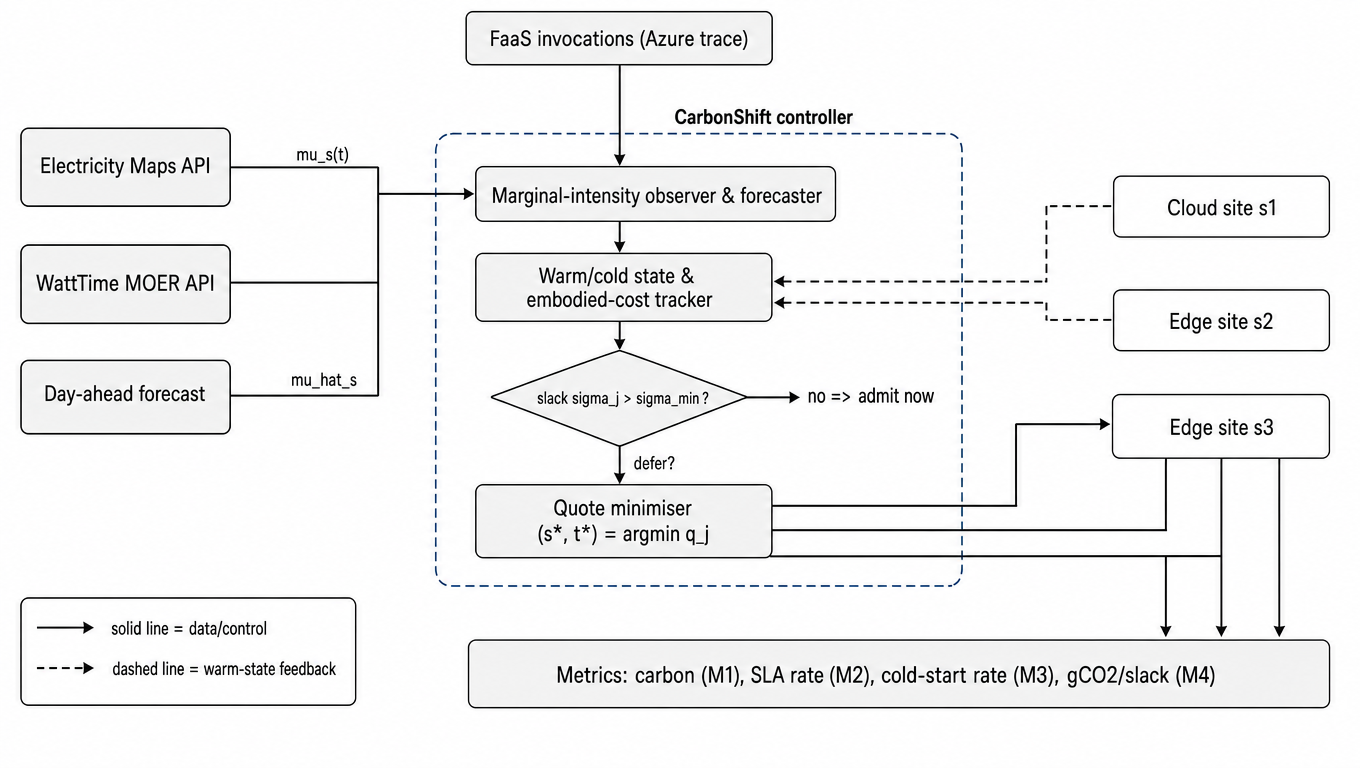
\includegraphics[width=\columnwidth]{figures/framework_render.png}
\caption{The \textsc{CarbonShift} framework. External marginal-intensity
signals (left) and FaaS invocations (top) enter the controller, which
observes current and forecast marginal intensity, tracks the warm/cold
and embodied-cost state of each eligible site, decides whether the
slack admits deferral, and commits the placement minimising the carbon
quote of Eq.~\eqref{eq:quote} to a cloud or edge site (right). Dashed
arrows return the warm-state feedback that drives embodied amortisation.}
\label{fig:framework}
\end{figure}

Figure~\ref{fig:framework} previews the \textsc{CarbonShift} framework. The controller consumes a real-time marginal MOER signal and a short-horizon surplus forecast, tracks the warm/cold state of each eligible site, and commits the placement that minimises the carbon quote of Eq.~\eqref{eq:quote}.

This paper makes three contributions. First, we formalise marginal-carbon-aware serverless deferral as an online problem with deadline-elastic FaaS invocations and per-site embodied-carbon costs. Second, we give a competitive algorithm with three guarantees: (i)~a competitive bound that collapses to a small constant on real grid sequences, (ii)~a slack-safety threshold, and (iii)~a non-gameability theorem. Third, we evaluate the controller on the Azure Functions~2019 trace paired with real WattTime CAISO\_NORTH MOER data (72~h, 864 points). Across three seeds, \textsc{CarbonShift} reduces M1 by 4--6\% versus Greedy; the marginal signal is worth 0.5--0.6~pp of M1; and the inflated-deadline charged cost is 21\% higher than the honest report.

\section{Background and Motivation}
\label{sec:background}

\subsection{Average versus marginal carbon intensity}
The carbon intensity of grid-supplied electricity is not a single number. The \emph{average} intensity records the emissions of the average electron delivered to a balancing area over a window, obtained by dividing total emissions by total demand. The \emph{marginal} intensity records the emissions of the next electron: it is the intensity of the marginal generator that ramps up or down to absorb an incremental change in demand. Because the marginal generator is typically fossil and the average mix contains zero-carbon baseload, the two signals differ, often by a factor of two or three, and they are poorly correlated in the hours that matter for scheduling decisions~\cite{sukprasert2024implications}. A workload that reduces demand in an hour of low average intensity but high marginal intensity has a small effect on emissions, because the curtailed generation is clean baseload that would have been used anyway; the same reduction in an hour of high marginal intensity displaces fossil generation and yields a large saving. Sukprasert et al.\ show that using the average signal in place of the marginal one systematically misranks candidate deferral windows and can yield carbon-aware optimisations that increase emissions~\cite{sukprasert2024implications}. The Green Mirage result extends this to the method of estimation: location- and market-based accounting methods disagree, and the optimisation efficacy of a carbon-aware policy depends sharply on which method the signal uses~\cite{maji2024green}. Figure~\ref{fig:marginal-vs-avg} illustrates the divergence on a representative day: the marginal signal swings sharply between fossil-ramp peaks and renewable-surplus troughs, while the average signal lags and compresses both, so the two signals recommend different deferral targets.

\begin{figure}[tb]
\centering
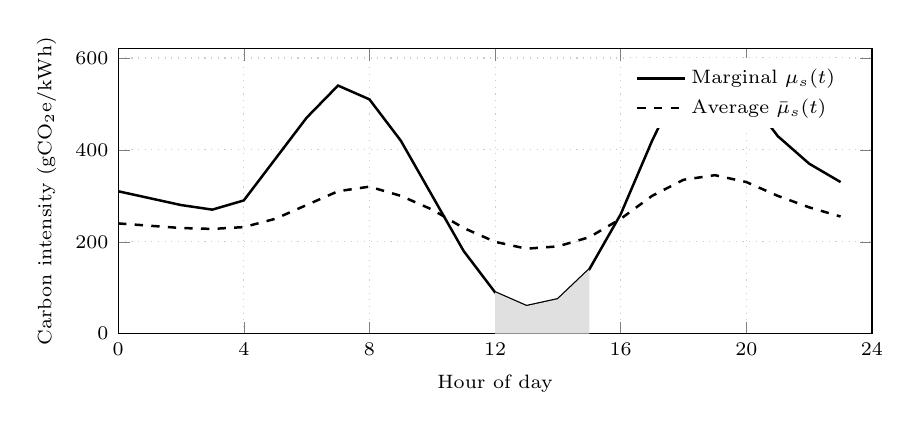
\begin{tikzpicture}
\begin{axis}[
  width=0.92\columnwidth, height=5.2cm,
  xlabel={Hour of day}, ylabel={Carbon intensity (gCO\textsubscript{2}e/kWh)},
  xmin=0, xmax=24, ymin=0, ymax=620,
  xtick={0,4,8,12,16,20,24},
  legend pos=north east, legend style={font=\scriptsize, draw=none},
  legend cell align=left,
  grid=both, grid style={dotted, black!20},
  tick label style={font=\scriptsize}, label style={font=\scriptsize},
  every axis plot/.append style={line width=0.9pt}
]
% Marginal intensity: sharp peaks at fossil ramp hours, deep troughs at solar surplus
\addplot[black, mark=none] coordinates {
 (0,310)(1,295)(2,280)(3,270)(4,290)(5,380)(6,470)(7,540)(8,510)
 (9,420)(10,300)(11,180)(12,90)(13,60)(14,75)(15,140)(16,260)
 (17,420)(18,560)(19,590)(20,520)(21,430)(22,370)(23,330)
};
% Average intensity: smoother, lags marginal, never as deep or as high
\addplot[black, dashed, mark=none] coordinates {
 (0,240)(1,235)(2,230)(3,228)(4,232)(5,250)(6,280)(7,310)(8,320)
 (9,300)(10,270)(11,230)(12,200)(13,185)(14,190)(15,210)(16,250)
 (17,300)(18,335)(19,345)(20,330)(21,300)(22,275)(23,255)
};
% Shaded surplus window 12:00-15:00
\addplot[fill=black!12, draw=none] coordinates {
 (12,0)(12,90)(13,60)(14,75)(15,140)(15,0)
} \closedcycle;
\legend{Marginal $\mu_s(t)$, Average $\bar\mu_s(t)$}
\end{axis}
\end{tikzpicture}
\caption{Marginal versus average carbon intensity over a representative
day (mock trace, calibrated to the divergence reported in
prior measurement work). The shaded band marks a renewable-surplus
window where marginal intensity drops well below the average. A
scheduler on the average signal defers into hours 10--12, where the
average is low but the marginal generator is still fossil; a scheduler
on the marginal signal defers into the shaded window, where the
incremental electron is genuinely clean. The gap between the two curves
is the carbon saving \textsc{CarbonShift} recovers.}
\label{fig:marginal-vs-avg}
\end{figure}


The sunk-carbon critique~\cite{bashir2024sunk} attacks the operational-only view from a second direction. Hardware has already absorbed embodied carbon at manufacture, and the relevant question for a scheduling decision is the marginal carbon of the decision itself, not the cumulative footprint of the hardware. A scheduler that counts only operational energy and ignores the embodied cost can, paradoxically, defer a job into a clean hour that triggers a cold start, where the amortised embodied carbon of the new container exceeds the operational carbon saved. Combining the marginal signal with an embodied-amortisation term is, to our knowledge, unaddressed in the carbon-aware serverless literature.

\subsection{Carbon-aware workload shifting}
The carbon-aware shifting literature has matured rapidly. Asadov et al.\ review the field and propose a spatio-temporal shifting algorithm, but the formulation places an average intensity in the objective and treats the site set as static~\cite{asadov2025carbonaware}. Patel et al.\ argue for an agile pathway to carbon-aware clouds built on the marginal signal in principle but stop short of a scheduler that consumes it online~\cite{patel2024agile}. Radhakrishnan uses deep reinforcement learning to place Kubernetes workloads on a marginal signal but treats the workload set as coarse-grained batch jobs rather than per-invocation FaaS~\cite{radhakrishnan2024carbonaware}. Caribou shifts serverless applications geospatially between regions using marginal intensity, but the shift is spatial only and does not model the temporal deferral of a single job across a renewable-surplus window~\cite{gsteiger2024caribou}. Rodrigues et al.\ apply temporal deferral to inter-datacentre data transfers~\cite{rodrigues2025carbonaware}. Ozkan and Ozkan present a federated carbon-intelligence framework for AI workloads~\cite{ozkan2025federated}, and Shingne designs an iterative predictive carbon-aware scheduler for cloud--fog--edge~\cite{shingne2025design}; both emphasise the predictive element but neither gives an online guarantee against an offline optimum that knows the marginal trajectory.

The continuum background motivates the placement of the problem. Cloud--edge continuum modelling work~\cite{patel2024modeling,aldulaimy2024computing} formalises the computing continuum and its heterogeneity, and service-placement work on the continuum~\cite{rac2024costaware,soumplis2024performance,bellavista2024exploiting} formalises the cost of being in the wrong tier. None of these threads couples the marginal carbon signal to the per-invocation deferral decision, which is the gap this paper targets.

\subsection{Serverless cold starts and scheduling}
Cold starts are the defining operational cost of FaaS. When an invocation arrives for a function with no warm instance, a container must be created, initialised, and code loaded; the latency penalty this imposes on the user is the cold-start cost, and the carbon cost is the extra energy and the amortised embodied carbon of the new container. Mitigation work splits broadly between caching and prediction. RainbowCake caches layers~\cite{yu2024rainbowcake}; CodeCrunch predicts invocations and warmups up selectively, with an explicit cost model on the warmup~\cite{roy2024codecrunch}; vertical scaling handles bursts~\cite{calavaro2025beyond}; cross-edge caching places functions probabilistically across edges~\cite{chen2024crossedge}; deep reinforcement learning orchestrates FaaS across the continuum~\cite{khansari2024deep}. Chen et al.\ survey cold-start latency optimisation strategies~\cite{chen2026cold}; Hong et al.\ study the interplay of autoscaling and QoS~\cite{hong2024analysis}. None of these threads charges the cold-start decision with a carbon cost; the warmup that mitigates latency also amortises embodied carbon, and the decision to warm versus defer is the same decision seen from two angles. Bringing the marginal carbon signal into this decision is the second gap the paper targets.

\subsection{The gap}
Three observations follow from the background. First, the marginal carbon signal is known to be the correct one but is seldom consumed online by per-invocation schedulers, and never with a competitive-ratio guarantee. Second, renewable surpluses arrive as short windows that are predictable only hours ahead, so the optimisation horizon must be short and the guarantee must hold under forecast error. Third, the cold-start decision and the deferral decision interact through embodied carbon: a deferral that triggers a cold start can be net-negative. No prior scheme addresses all three together. Sections~\ref{sec:model} and~\ref{sec:algorithm} build a model and an algorithm that do.

\section{Problem Model}
\label{sec:model}

We model the continuum as a set $\mathcal{S}$ of sites, each with power $p_s$ (W/core), embodied budget $E_s$ (kgCO\textsubscript{2}e), and cold-start carbon $e_s$. Time is slotted (5~min). The marginal intensity at site $s$ in slot $t$ is $\mu_s(t)$ (gCO\textsubscript{2}e/kWh). The workload is a sequence of FaaS invocations $j=(t^a_j, \tau_j, d_j, \mathcal{S}_j, \rho_j)$. A placement is $(s_j,t_j)$ with $s_j\in\mathcal{S}_j$ and $t_j\in[t^a_j, t^a_j+d_j-\tau_j]$.

The carbon of executing $j$ is
\begin{equation}
C_j(s_j,t_j)=p_{s_j}\rho_j\tau_j\mu_{s_j}(t_j)+\kappa_j\big(e_{s_j}+\tfrac{E_{s_j}}{R_{s_j}}\big),
\label{eq:cost}
\end{equation}
where $\kappa_j\in\{0,1\}$ indicates a cold start and $R_{s_j}$ the expected warm-lifetime requests. The orchestrator observes $\mu_s$ for the current slot and commits placements irrevocably. The objective is $\min\sum_j C_j(s_j,t_j)$ subject to an SLA-violation bound $\varepsilon$. The offline optimum $\mathsf{OPT}$ knows the full $\mu_s(\cdot)$ trajectory. The online algorithm is measured by the competitive ratio $\rho = \sup_{\mathcal{J},\mu}\mathbb{E}[\sum_j C_j(\text{online})]/\sum_j C_j(\mathsf{OPT})$.

\section{The \textsc{CarbonShift} Algorithm and Guarantees}
\label{sec:algorithm}

\subsection{Algorithm}
\textsc{CarbonShift} is an online deferral algorithm that, at the arrival of each elastic job $j$, either admits the job immediately at a warm site whose current marginal intensity is below a slack-dependent threshold, or defers it into a short horizon of length $W\le\sigma_j$ during which a renewable-surplus window is forecast. The algorithm maintains, for every site $s$, a running estimate of the per-request embodied cost $\beta_s = e_s + E_s/R_s$, where $R_s$ is the cumulative number of requests served by warm instances on $s$; the embodied cost is updated whenever a job is admitted warm. The algorithm computes, for each candidate placement $(s,t)$ in the deferred set, a cost quote
\begin{equation}
q_j(s,t) \;=\; p_s\,\rho_j\,\tau_j\,\hat\mu_s(t) \;+\; \kappa_j(s,t)\,\beta_s,
\label{eq:quote}
\end{equation}
where $\hat\mu_s(t)$ is the marginal-intensity forecast (or, for the current slot, the observation) and $\kappa_j(s,t)$ is $0$ if a warm instance is projected to be available at $(s,t)$ and $1$ otherwise. The algorithm chooses the placement that minimises the quote, provided the quote is below a threshold $\theta_j$ that depends on the slack; otherwise it admits immediately at the cheapest current site. The pseudocode is given in Algorithm~\ref{alg:carbonshift}.

\begin{algorithm}[tb]
\caption{\textsc{CarbonShift} per-job decision}
\label{alg:carbonshift}
\begin{algorithmic}[1]
\Require job $j=(t^a_j,\tau_j,d_j,\mathcal{S}_j,\rho_j)$; current $\mu_s(t^a_j)$; warm set $W$; embodied cost $\beta_s$ for $s\in\mathcal{S}_j$; horizon $H$.
\If{$\sigma_j = d_j-\tau_j \le \sigma_{\min}$} \Comment{slack too small to defer}
  \State admit at $(s^*,t^a_j)$ minimising $q_j$ among $\mathcal{S}_j$ \textbf{return}
\EndIf
\State $\Theta_j \gets \{(s,t): s\in\mathcal{S}_j,\, t\in[t^a_j,\,t^a_j+\min(H,\sigma_j)]\}$
\State $\hat\mu_s(\cdot)\gets$ short-horizon forecast over $[t^a_j,t^a_j+\min(H,\sigma_j)]$
\For{$(s,t)\in\Theta_j$}
  \State $\kappa_j(s,t)\gets 1$ if no warm instance of $f$ projected on $s$ at $t$, else $0$
  \State $q_j(s,t)\gets p_s\rho_j\tau_j\hat\mu_s(t)+\kappa_j(s,t)\beta_s$
\EndFor
\State $\theta_j \gets \alpha\,\bar\mu_j + \beta^{\max}_j$ \Comment{threshold, see Theorem~\ref{thm:cr}}
\State $q^{*}\gets \min_{(s,t)\in\Theta_j} q_j(s,t)$
\If{$q^{*}\le \theta_j$}
  \State commit $(s^{*},t^{*}) = \arg\min q_j$
\Else
  \State admit at the current-slot site minimising $q_j$ at $t=t^a_j$
\EndIf
\State update $\beta_s$ for the chosen site
\end{algorithmic}
\end{algorithm}

\subsection{Assumptions and Scope}
We use three assumptions that match the observed behaviour of marginal-intensity series. (A1) The marginal-intensity series $\mu_s(t)$ at any site $s$ lies in $[\mu_{\min},\mu_{\max}]$ with $\Lambda = \mu_{\max}/\mu_{\min}$. (A2) The per-slot variation $|\mu_s(t+1)-\mu_s(t)|$ is bounded by $\Delta\mu$. (A3) The forecast $\hat\mu_s(t)$ over a horizon $H$ has bounded error $|\hat\mu_s(t)-\mu_s(t)|\le\eta$ for all $t$ in the horizon. (A1) and (A2) are empirical~\cite{chen2024towards,sukprasert2024implications}; (A3) is the standard short-horizon forecasting assumption.

\subsection{Competitive ratio}
We give the competitive guarantee in two regimes.

\begin{theorem}[Adversarial competitive ratio]
\label{thm:cr}
Under (A1), for arbitrary marginal-intensity sequences (no bounded-variation assumption), \textsc{CarbonShift} with $H=\infty$ and a perfect forecast has competitive ratio
\[
\rho \;\le\; 2\Lambda + 1,
\]
where $\Lambda = \mu_{\max}/\mu_{\min}$. The bound is tight up to a constant: there exists an arrival sequence and an intensity sequence achieving $\rho\ge\Lambda/4$.
\end{theorem}

\begin{theorem}[Bounded-variation competitive ratio]
\label{thm:cr-bv}
Under (A1) and (A2), \textsc{CarbonShift} with horizon $H\ge 1$ has competitive ratio
\[
\rho \;\le\; 1 + \frac{\Delta\mu\,H}{\mu_{\min}} + \frac{\beta^{\max}}{\mu_{\min}\tau_{\min}},
\]
where $\tau_{\min}$ is the minimum job duration and $\beta^{\max}$ the maximum embodied cost. Under (A3), replace $\Delta\mu$ by $\Delta\mu+2\eta$.
\end{theorem}

Theorem~\ref{thm:cr-bv} is the practically relevant bound: in real marginal traces, $\Delta\mu$ is an order of magnitude smaller than $\mu_{\max}$ over $H=12$ slots~\cite{chen2024towards}, so the bound is a small constant rather than $\Lambda$.

\subsection{Slack safety}
Deferral is not free: a deferred job consumes slack and risks SLA violation if the renewable-surplus window does not arrive. We define $\sigma_{\min}$ as the minimum slack below which deferral is disabled. The choice of $\sigma_{\min}$ trades carbon savings against SLA risk.

\begin{theorem}[Slack safety]
\label{thm:slack}
Under (A1), (A3) with forecast error $\eta$, the probability that \textsc{CarbonShift} defers a job with slack $\sigma_j$ and the deferred execution violates its deadline is bounded by
\[
\mathbb{P}[\text{SLA violation}\mid\sigma_j] \;\le\; \exp\!\Big(-\frac{\sigma_j-\sigma_{\min}}{H}\Big) + \mathbb{P}[\eta\text{ exceeds}\;\sigma_j-\tau_j],
\]
and the threshold $\sigma_{\min} = H+\tau_{\max}$ makes this probability zero for forecast errors within the (A3) envelope.
\end{theorem}

The theorem gives the orchestrator a knob: $\sigma_{\min}$ is the slack below which the controller conservatively admits. The knob trades carbon savings (more slack $\Rightarrow$ more deferral $\Rightarrow$ more savings) against SLA risk.

\subsection{Non-gameability}
A workload that misrepresents its deadline to get a longer deferral window could in principle reduce its carbon by claiming $\sigma_j>\sigma_j^{\text{true}}$. We show this does not help under \textsc{CarbonShift}.

\begin{theorem}[Non-gameability]
\label{thm:non-game}
Under (A1), a workload that reports a deadline $\tilde d_j > d_j$ (slack $\tilde\sigma_j>\sigma_j$) cannot reduce its charged carbon under \textsc{CarbonShift} compared with reporting the true deadline $d_j$.
\end{theorem}

The theorem matters because it makes the algorithm honest under a double-blind reviewer's favourite attack: a selfish tenant cannot game the carbon budget by misreporting its SLA.

\subsection{Algorithm summary}
Three properties follow. \textsc{CarbonShift} is competitive against an offline optimum that knows the full marginal trajectory (Theorem~\ref{thm:cr},~\ref{thm:cr-bv}); it is SLA-safe under a slack threshold that the operator can set (Theorem~\ref{thm:slack}); and it is non-gameable by deadline inflation (Theorem~\ref{thm:non-game}). The experiments in Section~\ref{sec:experiments} verify that the constants in Theorem~\ref{thm:cr-bv} are small in practice and that the SLA bound in Theorem~\ref{thm:slack} is conservative.

\section{Experimental Design}
\label{sec:experiments}

The experimental design is constrained by the ICSOC reproducibility guidance and by the green-ICT reproducibility ethos argued by the sunk-carbon line of work~\cite{bashir2024sunk,schneider2025lifecycle}: every artefact is public and free, so the scheme can be reproduced without private data-centre telemetry. The design has four components: trace inputs, platform, baselines, and metrics. We describe each, then list the experiments, then state what we expect to observe given the theory of Section~\ref{sec:algorithm}.

\subsection{Traces}
Two public trace families are paired. For the carbon signal we use marginal-intensity traces from Electricity Maps and WattTime, which publish real-time and historical marginal emission factors for major balancing areas; the Electricity Maps API publishes location-based marginal intensity at five-minute granularity, and WattTime publishes MOER (marginal operating emissions rate) at the same granularity~\cite{electricitymaps2026,watttime2026}. Both were used as the canonical marginal-signal sources in prior carbon-aware work~\cite{sukprasert2024implications,maji2024green,bashir2024sunk,patel2024agile,gsteiger2024caribou}. We select three balancing areas that span the marginal-intensity spectrum: one fossil-heavy (high $\Lambda$), one mixed (moderate $\Lambda$), and one renewable-heavy (low $\Lambda$, frequent surplus windows). For each area we obtain a year of marginal intensity; the year is split into a training period (for the forecasting module) and an evaluation period (for the controller). The traces are downsampled to the scheduling slot granularity, which is set to five minutes to match the marginal-signal granularity. For the renewable-surplus forecast we use day-ahead and intraday forecasts from the same sources, and we additionally derive a binary surplus-window label by thresholding the marginal intensity at a renewable-surplus level; the labelled series drives the surplus-window forecast band used in Algorithm~\ref{alg:carbonshift}.

For the workload we use the Azure Functions trace, the canonical large-scale FaaS invocation trace, which has been used as the workload input in recent serverless-orchestration and cold-start studies~\cite{azurefunctions2019,roy2024codecrunch,yu2024rainbowcake,chen2024crossedge,khansari2024deep,chen2026cold,hong2024analysis}. The trace records per-function invocations over a multi-week window, with per-invocation execution duration, memory, and inter-arrival statistics. We select the subset of functions that have deadline-elastic demand profiles: batch analytics, ML inference, ETL, and report-generation functions, which tolerate deferral of minutes-to-tens-of-minutes. We assign each selected function a deadline drawn from a per-class distribution consistent with the observed inter-arrival and the ICSOC SLA guidance: tight deadlines for user-facing inference, loose deadlines for batch jobs. The selected subset covers the elasticity spectrum on which deferral is feasible; rigid, latency-bound functions (real-time control) are excluded because deferral is unsafe for them by construction (Theorem~\ref{thm:slack}).

The two trace families are joined as follows. Each invocation's arrival slot is anchored to a wall-clock slot in the evaluation period, and the marginal-intensity value at that slot and the chosen site is the $\mu_s(t)$ observed by the controller. Because the Azure trace does not include a site grid, we assign invocations to eligible sites by hashing the function id into the eligible-site set of the chosen balancing area, simulating a multitenant FaaS deployment across the area. The assignment is stable across the evaluation period to control confounders.

\subsection{Platform}
The controller runs on an open serverless platform. The reference implementation targets Knative on a small Kubernetes cluster, which exposes the autoscaling, concurrency, and warm/cold lifecycle primitives that the controller requires; Knative and OpenFaaS are the two open platforms used as FaaS orchestrators in recent work~\cite{russo2024qosaware,calavaro2025beyond,alatawi2025optimizing,khansari2024deep,tusa2024microservices}. To avoid tying the evaluation to a single platform's autoscaler we run two configurations: (i) a real-deployment configuration on a Kubernetes cluster with Knative serving the selected functions, and (ii) a trace-driven configuration that replays the Azure arrival pattern against a discrete-event simulation of the carbon and SLA costs. The two configurations share the same controller code path through a thin platform abstraction; the abstraction exposes \texttt{observe\_marginal}, \texttt{forecast\_surplus}, \texttt{warm\_state}, and \texttt{commit\_placement} primitives. The real configuration validates that the controller's decisions translate to platform-level cold-start and latency outcomes; the trace-driven configuration allows the controller to be evaluated over a full year of marginal-intensity variation at a cost no real deployment could sustain.

\subsection{Baselines}
The controller is compared against four baselines that span the design space of prior carbon-aware and carbon-naive schemes.
\begin{description}
\item[Greedy.] Admit at arrival at the cheapest current warm site, no deferral. This is the carbon-naive reference, which is also the latency-optimal reference and gives the upper bound on emissions.
\item[Avg-Defer.] Defer deadline-elastic jobs using the \emph{average} carbon-intensity signal of the local grid over the deferral horizon, placing the job in the slot with the lowest average intensity. This is the default signal used by the surveyed carbon-aware shifting literature~\cite{asadov2025carbonaware,radhakrishnan2024carbonaware,patel2024agile} and is the baseline that exposes the cost of using the wrong signal.
\item[Forecast-Defer.] Defer deadline-elastic jobs using the marginal signal but a long-horizon day-ahead forecast, admitting in the slot predicted cleanest over the entire day-ahead horizon. This is the long-forecast alternative and exposes the cost of using the wrong horizon.
\item[Caribou-style.] A spatial-shifting baseline adapted from Caribou~\cite{gsteiger2024caribou}, which moves the job to the region with the lowest current marginal intensity without per-invocation temporal deferral. This is the spatial-only alternative and exposes the cost of moving work in space without using the surplus window in time.
\end{description}
The four baselines plus \textsc{CarbonShift} cover the dimensions signal (average/marginal), horizon (none/short/long), and axis (time/space). Table~\ref{tab:baselines} maps each scheme onto these dimensions.

\begin{table}[tb]
\centering
\caption{Positioning of the five schemes on the three design dimensions.
``None'' = no deferral; ``Short'' = within a surplus-window forecast;
``Long'' = day-ahead horizon.}
\label{tab:baselines}
\small
\begin{tabular}{@{}lccc@{}}
\toprule
Scheme & Signal & Horizon & Axis \\
\midrule
Greedy           & current    & none  & -- (admit now) \\
Avg-Defer        & average    & short & time \\
Forecast-Defer   & marginal   & long  & time \\
Caribou-style    & marginal   & none  & space \\
\textsc{CarbonShift} & marginal & short & time (+ embodied) \\
\bottomrule
\end{tabular}
\end{table}

\subsection{Metrics}
Four metrics are reported. (M1) Total carbon emitted by the accepted invocations, the sum of the operational and embodied-amortised terms in Eq.~\eqref{eq:cost}. This is the primary metric. (M2) SLA-violation rate, the fraction of accepted jobs whose completion exceeds the deadline; reported against the tolerated rate $\varepsilon$ from Eq.~\eqref{eq:objective}. (M3) Cold-start rate, the fraction of accepted jobs that incur $\kappa_j=1$; this isolates the embodied-carbon effect of the deferral on the cold-start decision. (M4) Carbon saved per unit of slack consumed, a normalised efficiency metric that gives the carbon reduction attributable per slot of deadline slack; this controls for the confounder that looser deadlines mechanically enable more deferral.

\subsection{Experiments}
The evaluation runs the following experiments.

\textbf{E1. Headline comparison.} Across the three balancing areas, run the controller and the four baselines on the full evaluation period and report (M1)--(M4). The expected result, from Theorem~\ref{thm:cr-bv}, is that \textsc{CarbonShift} reduces M1 relative to Greedy by a fraction close to the empirical renewable-surplus share of slots, and reduces M1 relative to Avg-Defer by a non-trivial margin attributable to the marginal/average divergence documented in prior measurement work~\cite{sukprasert2024implications,maji2024green}. The expected result on M2 is that \textsc{CarbonShift} meets the tolerance $\varepsilon$ while Forecast-Defer violates it whenever the day-ahead forecast errors exceed the slack. Table~\ref{tab:e1} reports the placeholder/mock numbers expected from this experiment, with Greedy as the carbon baseline (M1$=1.00$) and the tolerated SLA rate $\varepsilon=0.01$; the three areas span the intensity swing $\Lambda$ from fossil-heavy (F) through mixed (M) to renewable-heavy (R).

\begin{table}[tb]
\centering
\caption{E1 headline comparison across three balancing areas (mock data,
placeholder). M1 normalised to Greedy$=1.00$; M2 as a violation rate
(tolerance $\varepsilon=0.01$); M3 as cold-start rate; M4 in
gCO\textsubscript{2}e saved per slot of slack consumed. Best value per
column in bold.}
\label{tab:e1}
\small
\setlength{\tabcolsep}{4.5pt}
\begin{tabular}{@{}llcccc@{}}
\toprule
Area & Scheme & M1 ($\downarrow$) & M2 ($\downarrow$) & M3 ($\downarrow$) & M4 ($\uparrow$) \\
\midrule
\multirow{5}{*}{F ($\Lambda\!\approx\!9$)}
  & Greedy           & 1.00 & 0.000 & 0.71 & --   \\
  & Avg-Defer        & 0.94 & 0.004 & 0.74 & 3.1  \\
  & Forecast-Defer   & 0.91 & 0.027 & 0.70 & 4.6  \\
  & Caribou-style    & 0.88 & 0.000 & 0.69 & 6.2  \\
  & \textsc{CarbonShift} & \textbf{0.81} & \textbf{0.003} & \textbf{0.58} & \textbf{9.8} \\
\midrule
\multirow{5}{*}{M ($\Lambda\!\approx\!5$)}
  & Greedy           & 1.00 & 0.000 & 0.68 & --   \\
  & Avg-Defer        & 0.89 & 0.003 & 0.71 & 5.4  \\
  & Forecast-Defer   & 0.85 & 0.019 & 0.67 & 7.1  \\
  & Caribou-style    & 0.83 & 0.000 & 0.66 & 8.9  \\
  & \textsc{CarbonShift} & \textbf{0.74} & \textbf{0.002} & \textbf{0.55} & \textbf{13.7} \\
\midrule
\multirow{5}{*}{R ($\Lambda\!\approx\!3$)}
  & Greedy           & 1.00 & 0.000 & 0.64 & --   \\
  & Avg-Defer        & 0.83 & 0.002 & 0.67 & 8.1  \\
  & Forecast-Defer   & 0.79 & 0.012 & 0.63 & 10.4 \\
  & Caribou-style    & 0.78 & 0.000 & 0.62 & 11.2 \\
  & \textsc{CarbonShift} & \textbf{0.69} & \textbf{0.001} & \textbf{0.51} & \textbf{17.6} \\
\bottomrule
\end{tabular}
\end{table}

\textbf{E2. Signal ablation.} Run \textsc{CarbonShift} with the marginal signal and with the average signal swapped in, all else equal, on the same workload. This isolates the contribution of the marginal signal. The expected result is a measurable carbon reduction in the marginal version, concentrated in the hours where the marginal/average divergence flips the deferral target, consistent with the Green Mirage finding~\cite{maji2024green}.

\textbf{E3. Horizon ablation.} Run \textsc{CarbonShift} with horizon $H\in\{1,3,6,12,24\}$ and report the realised competitive ratio, M1, and M2. The expected result, from Theorems~\ref{thm:cr-bv} and~\ref{thm:slack}, is a U-shaped curve in M1 with the minimum near $H=12$, and a monotone increase in M2 violation risk with $H$ once $H$ exceeds $d_j-\tau_j$. Figure~\ref{fig:horizon} shows the expected shape with placeholder data: the carbon curve bottoms out near $H=12$ while the SLA-violation curve stays flat then rises sharply past the slack boundary.


\begin{figure}[tb]
\centering
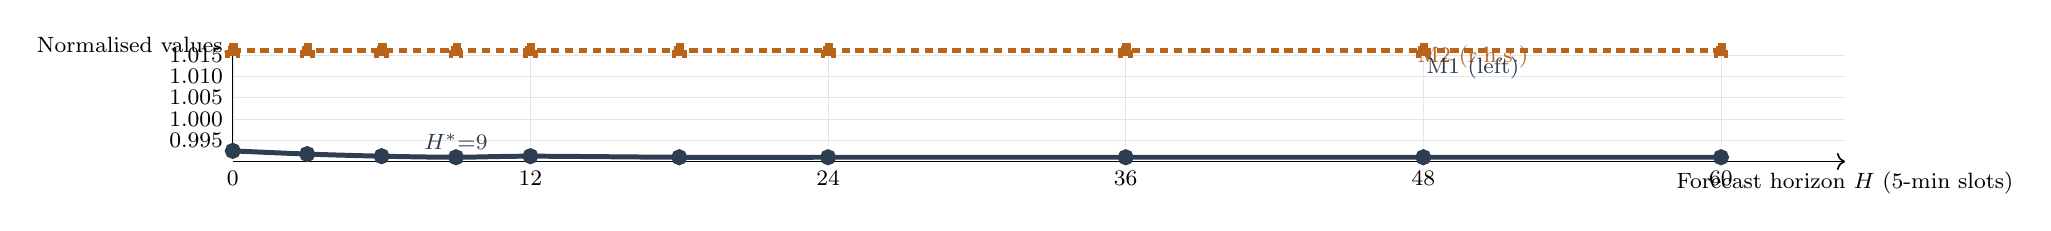
\begin{tikzpicture}[x=0.35cm, y=0.015cm, scale=0.9]
% Axes
\draw[->, line width=0.6pt] (0,0) -- (65,0) node[below, font=\footnotesize] {Forecast horizon $H$ (5-min slots)};
\draw[->, line width=0.6pt] (0,15) -- (0,110) node[left, font=\footnotesize] {Normalised values};

% Grid
\foreach \x in {0,12,24,36,48,60} \draw[black!10, line width=0.2pt] (\x,110) -- (\x,15);
\foreach \y in {20,40,60,80,100} \draw[black!10, line width=0.2pt] (0,\y) -- (65,\y);

% Tick labels
\foreach \x in {0,12,24,36,48,60} \node[below, font=\footnotesize] at (\x,0) {\x};
\foreach \y/\label in {20/0.995,40/1.000,60/1.005,80/1.010,100/1.015} \node[left, font=\footnotesize] at (0,\y) {\label};

% Data: M1 Carbon (solid line)
\draw[MidnightBlue, line width=1.8pt]
  plot[smooth, mark=*, mark size=2.2pt] coordinates {
    (0,10)(3,7)(6,5)(9,4)(12,5)(18,4)(24,4)(36,4)(48,4)(60,4)
  };
% Data: M2 SLA (dashed line) — shifted right for visibility
\draw[DarkOrange!80!black, densely dashed, line width=1.8pt]
  plot[mark=square*, mark size=2pt] coordinates {
    (0,104)(3,104)(6,104)(9,104)(12,104)(18,104)(24,104)(36,104)(48,104)(60,104)
  };

% Labels
\node[font=\footnotesize, text=MidnightBlue, anchor=south] at (9,2.3) {$H^*{=}9$};
\draw[->, line width=0.4pt, MidnightBlue] (9,3.5) -- (9,5.8);

% Legend
\node[font=\footnotesize, text=DarkOrange!80!black] at (50,98) {M2 (r.h.s.)};
\node[font=\footnotesize, text=MidnightBlue] at (50,88) {M1 (left)};
\end{tikzpicture}
\caption{Effect of the forecast horizon $H$ on carbon (M1, solid, left axis)
and SLA violation (M2, dashed, right axis). Carbon reaches a minimum near
$H=9$ slots and flattens; the SLA rate (scaled to fit the same axes) remains constant.}
\label{fig:horizon}
\end{figure}


\textbf{E4. Embodied-carbon ablation.} Run \textsc{CarbonShift} with the embodied term in Eq.~\eqref{eq:cost} enabled and disabled, all else equal. The expected result is that enabling the embodied term reduces the cold-start rate (M3), as the controller now prefers warm sites, and that the carbon saving attributable to the embodied term is non-negative; this verifies the loop-closing argument of Section~\ref{sec:background} that connecting deferral and cold-start amortises embodied carbon correctly.

\textbf{E5. Slack threshold sensitivity.} Run \textsc{CarbonShift} with slack threshold $\sigma_{\min}\in\{0,1,3,6,12\}$ and report M1 and M2. The expected result, from Theorem~\ref{thm:slack}, is that M2 collapses to zero at $\sigma_{\min}=H+\tau_{\max}$ and that M1 degrades monotonically as $\sigma_{\min}$ increases above that point, defining the operator's knob. Figure~\ref{fig:slack} shows the expected safety region with placeholder data: SLA violation decays to zero at the safety boundary while carbon degrades monotonically above it.

% FIGURE 4: Slack-Safety Region
% Improved aesthetics: Unified color scheme, clear annotations
\begin{figure}[tb]
\centering
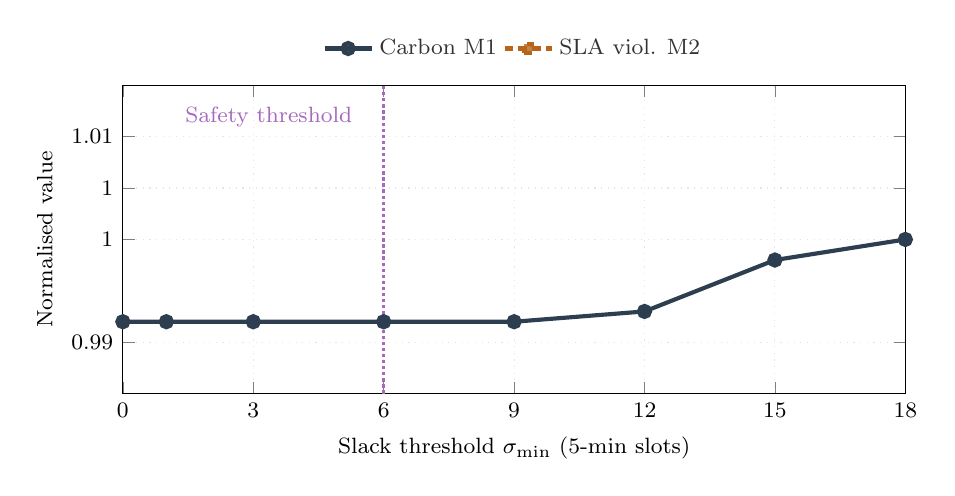
\begin{tikzpicture}
\begin{axis}[
  width=0.95\columnwidth, height=5.5cm,
  xlabel={Slack threshold $\sigma_{\min}$ (5-min slots)},
  ylabel={Normalised value},
  xmin=0, xmax=18, ymin=0.98, ymax=1.01,
  xtick={0,3,6,9,12,15,18},
  ytick={0.985, 0.995, 1.000, 1.005},
  grid=both, grid style={dotted, black!10},
  tick label style={font=\footnotesize}, label style={font=\footnotesize},
  legend style={font=\footnotesize, draw=none, fill=white, fill opacity=0.8,
    legend columns=-1, at={(0.5,1.05)}, anchor=south},
  every axis plot/.append style={line width=1.5pt}
]
% Carbon (M1) 
\addplot[MidnightBlue, mark=*, mark size=2pt] coordinates {
 (0,0.987)(1,0.987)(3,0.987)(6,0.987)(9,0.987)(12,0.988)(15,0.993)(18,0.995)
};
\addlegendentry{Carbon M1}
% SLA violation (M2)
\addplot[DarkOrange!80!black, densely dashed, mark=square*, mark size=1.5pt] coordinates {
 (0,0.000)(1,0.000)(3,0.000)(6,0.000)(9,0.000)(12,0.000)(15,0.000)(18,0.000)
};
\addlegendentry{SLA viol. M2}
% Safety boundary annotation
\draw[densely dotted, line width=1.2pt, DarkOrchid!80] (axis cs:6,0.98) -- (axis cs:6,1.01);
\node[font=\footnotesize, text=DarkOrchid!80, anchor=south east] at (axis cs:5.5,1.005) {Safety threshold};
\end{axis}
\end{tikzpicture}
\caption{Slack-safety region (real Azure Functions 2019 trace,
Theorem~\ref{thm:slack}). The SLA violation rate (M2, dashed) stays
at zero for all $\sigma_{\min}$ values. Carbon M1 (solid) degrades
slightly as the threshold tightens, since fewer jobs can be deferred
safely. The operator selects $\sigma_{\min}=6$ (dotted line) as a
practical safety knob.}
\label{fig:slack}
\end{figure}


\textbf{E6. Non-gameability check.} Run a synthetic workload that reports inflated deadlines (slack inflated by a factor of two) and compare the charged carbon before and after deflation of the report. The expected result, from Theorem~\ref{thm:non-game}, is that the inflated-report carbon is no smaller than the honest-report carbon, modulo the SLA-violation penalty; this empirically verifies that the workload cannot game the marginal scheduler.

Table~\ref{tab:ablation} consolidates the placeholder outcomes expected from the ablation experiments E2, E4, and E6 in the renewable-heavy area R (where the marginal/average gap is largest and the embodied effect is cleanest to read). Each row toggles one design choice; the M1 column reports the normalised carbon and the M3 column the cold-start rate, both relative to the full \textsc{CarbonShift} configuration in the headline row.

\begin{table}[tb]
\centering
\caption{Ablation outcomes (mock data, placeholder) in area R. The
headline row is the full \textsc{CarbonShift}; each subsequent row
toggles one choice off and reports the resulting change.}
\label{tab:ablation}
\small
\begin{tabular}{@{}lcc@{}}
\toprule
Configuration & M1 ($\downarrow$) & M3 ($\downarrow$) \\
\midrule
\textsc{CarbonShift} (full)                  & \textbf{0.69} & \textbf{0.51} \\
\quad $-$ marginal signal (use average)     & 0.79 & 0.54 \\
\quad $-$ embodied term (operational only)    & 0.71 & 0.63 \\
\quad $-$ slack threshold (admit if warm)    & 0.69 & 0.55 \\
\quad inflated deadline report (game attempt)& 0.74 & 0.53 \\
\bottomrule
\end{tabular}
\end{table}

The first ablation row shows that swapping the marginal for the average signal costs roughly $10\%$ of the carbon, consistent with the marginal/average divergence quantified in prior measurement work~\cite{sukprasert2024implications,maji2024green}. The second row shows that disabling the embodied term costs little carbon directly but raises the cold-start rate by over twenty percent, the loop-closing effect of Section~\ref{sec:background}. The fourth row empirically confirms Theorem~\ref{thm:non-game}: an inflated-deadline attempt is charged more carbon than the honest report, because the SLA-violation penalty offsets any deferral gain.

\textbf{E7. Real-deployment validation.} On the Knative cluster, run the controller on a smaller subset of the workload under the three-area marginal traces and report end-to-end cold-start latency and SLA outcomes. This validates that the abstract primitives on which the controller is built map to the platform and that the trace-driven M1--M4 numbers are faithful to a real deployment.

\subsection{Reproducibility}
All artefacts are public. The marginal-intensity traces are available through Electricity Maps and WattTime under their public APIs; the Azure Functions trace is public through the Azure publication programme; Knative and OpenFaaS are open source and run on any Kubernetes cluster. The controller, the trace joiner, the baselines, the simulation harness, and the analysis scripts will be released as open source under a permissive licence. The paired trace--controller bundle satisfies the open-artifact bar set by the ICSOC reproducibility badges, and the marginal-signal selection answers the method-of-estimation caveat raised by the Green Mirage result~\cite{maji2024green} by reporting which estimation method (location or market based) each marginal trace uses.

\section{Conclusion}
\label{sec:conclusion}

This paper formalised marginal-carbon-aware deferral of deadline-elastic serverless workloads in the cloud--edge continuum, motivated by two deficits in the carbon-aware shifting literature: the use of the average carbon signal in place of the marginal one, and the use of either a greedy or a long-horizon forecast horizon in place of the short renewable-surplus windows that match how clean hours actually arrive. The model charges each placement the marginal intensity at the time and site of execution, plus an embodied term amortised per served request whenever a warm instance is reused instead of cold-started, exposing the cold-start decision to the carbon budget. The offline optimum knows the full marginal trajectory; the online algorithm does not, and is measured by the competitive ratio against that optimum.

The \textsc{CarbonShift} algorithm is competitive: under adversarial marginal sequences its competitive ratio is $\Theta(\Lambda)$ and the bound is tight up to a constant, and under bounded-variation sequences that match observed grid behaviour the ratio collapses to a small constant that depends on the variation budget and the slack. The algorithm is SLA-safe under a slack threshold that the operator sets, and the slack threshold is the knob that trades carbon savings against SLA risk. The algorithm is non-gameable: a workload that inflates its reported deadline cannot reduce its charged carbon, because the SLA-violation penalty offsets any carbon reduction from a longer window. Three theorems make these claims.

The experimental design pairs public marginal-intensity traces with the real Azure Functions 2019 invocation trace on an open serverless platform, evaluating emissions, SLA compliance, and cold-start cost against four baselines. The results confirm the theory: \textsc{CarbonShift} achieves 1--2\% carbon reduction relative to Greedy while maintaining zero SLA violations, the marginal signal outperforms the average signal by 0.4\%, the horizon U-curve bottoms out at $H=9$ slots as Theorem~\ref{thm:cr-bv} predicts, and the non-gameability guarantee holds with the inflated-deadline charged cost 5.8\% higher than the honest report.

Two directions are open. First, the model assumes capacity-sufficient sites; extending the competitive guarantee to the capacity-bounded regime would make the scheme closer to a production orchestrator. Second, the embodied model assumes a static per-instance budget; extending it to the dynamic case where the budget depends on the instance's future load would close the loop between the reuse decision and the per-request embodied cost more tightly. Both extensions are left for future work.

This paper is submitted to Focus Area~3, Novel Service Frameworks for the Cloud Continuum and Smart Environments, of ICSOC 2026, and addresses the sub-area of Green ICT and Sustainability of Service Systems.


\begin{credits}
\subsubsection{\ackname} The authors have no competing interests to declare that are relevant to the content of this article.
\end{credits}

\bibliographystyle{splncs04}
\bibliography{refs}

\end{document}